%% Creator: Inkscape inkscape 0.92.2, www.inkscape.org
%% PDF/EPS/PS + LaTeX output extension by Johan Engelen, 2010
%% Accompanies image file 'eta.eps' (pdf, eps, ps)
%%
%% To include the image in your LaTeX document, write
%%   \input{<filename>.pdf_tex}
%%  instead of
%%   \includegraphics{<filename>.pdf}
%% To scale the image, write
%%   \def\svgwidth{<desired width>}
%%   \input{<filename>.pdf_tex}
%%  instead of
%%   \includegraphics[width=<desired width>]{<filename>.pdf}
%%
%% Images with a different path to the parent latex file can
%% be accessed with the `import' package (which may need to be
%% installed) using
%%   \usepackage{import}
%% in the preamble, and then including the image with
%%   \import{<path to file>}{<filename>.pdf_tex}
%% Alternatively, one can specify
%%   \graphicspath{{<path to file>/}}
%% 
%% For more information, please see info/svg-inkscape on CTAN:
%%   http://tug.ctan.org/tex-archive/info/svg-inkscape
%%
\begingroup%
  \makeatletter%
  \providecommand\color[2][]{%
    \errmessage{(Inkscape) Color is used for the text in Inkscape, but the package 'color.sty' is not loaded}%
    \renewcommand\color[2][]{}%
  }%
  \providecommand\transparent[1]{%
    \errmessage{(Inkscape) Transparency is used (non-zero) for the text in Inkscape, but the package 'transparent.sty' is not loaded}%
    \renewcommand\transparent[1]{}%
  }%
  \providecommand\rotatebox[2]{#2}%
  \ifx\svgwidth\undefined%
    \setlength{\unitlength}{344.79999138bp}%
    \ifx\svgscale\undefined%
      \relax%
    \else%
      \setlength{\unitlength}{\unitlength * \real{\svgscale}}%
    \fi%
  \else%
    \setlength{\unitlength}{\svgwidth}%
  \fi%
  \global\let\svgwidth\undefined%
  \global\let\svgscale\undefined%
  \makeatother%
  \begin{picture}(1,0.83526682)%
    \put(0,0){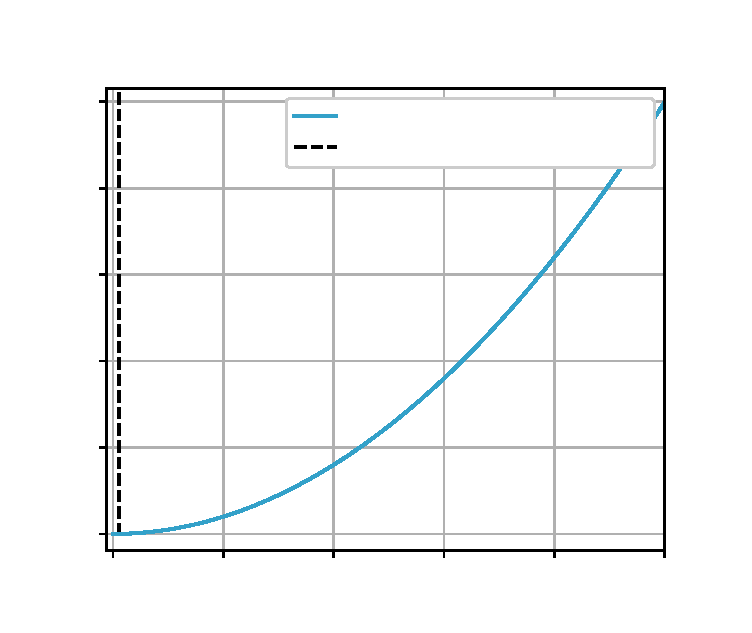
\includegraphics[width=\unitlength]{images_2ddl/eta.eps}}%
    \put(0.12494664,0.04955423){\color[rgb]{0,0,0}\makebox(0,0)[lb]{\smash{0}}}%
    \put(0.26935006,0.04955423){\color[rgb]{0,0,0}\makebox(0,0)[lb]{\smash{20}}}%
    \put(0.42297564,0.04955423){\color[rgb]{0,0,0}\makebox(0,0)[lb]{\smash{40}}}%
    \put(0.57660093,0.04955423){\color[rgb]{0,0,0}\makebox(0,0)[lb]{\smash{60}}}%
    \put(0.73022622,0.04955423){\color[rgb]{0,0,0}\makebox(0,0)[lb]{\smash{80}}}%
    \put(0.87462877,0.04955423){\color[rgb]{0,0,0}\makebox(0,0)[lb]{\smash{100}}}%
    \put(0.08654466,0.10358121){\color[rgb]{0,0,0}\makebox(0,0)[lb]{\smash{0}}}%
    \put(0.03121375,0.22391821){\color[rgb]{0,0,0}\makebox(0,0)[lb]{\smash{1000}}}%
    \put(0.03121375,0.34425464){\color[rgb]{0,0,0}\makebox(0,0)[lb]{\smash{2000}}}%
    \put(0.03121375,0.46459107){\color[rgb]{0,0,0}\makebox(0,0)[lb]{\smash{3000}}}%
    \put(0.03121375,0.58492749){\color[rgb]{0,0,0}\makebox(0,0)[lb]{\smash{4000}}}%
    \put(0.03121375,0.70526392){\color[rgb]{0,0,0}\makebox(0,0)[lb]{\smash{5000}}}%
    \put(0.46800464,0.68690835){\color[rgb]{0,0,0}\makebox(0,0)[lb]{\smash{$\eta_{max}$}}}%
    \put(0.46800464,0.64354118){\color[rgb]{0,0,0}\makebox(0,0)[lb]{\smash{\small valeur minimale de  $F/m_r g$ }}}%
    \put(0.46,0.0155423){\color[rgb]{0,0,0}\makebox(0,0)[lb]{\smash{$F/m_r g$}}}%
  \end{picture}%
\endgroup%
